\documentclass[]{report}
\usepackage[T1]{fontenc}
\usepackage{lmodern}
\usepackage{amssymb,amsmath}
\usepackage{abstract}
\usepackage{ifxetex,ifluatex}
\usepackage{fixltx2e} % provides \textsubscript
% use upquote if available, for straight quotes in verbatim environments
\IfFileExists{upquote.sty}{\usepackage{upquote}}{}
\ifnum 0\ifxetex 1\fi\ifluatex 1\fi=0 % if pdftex
  \usepackage[utf8]{inputenc}
\else % if luatex or xelatex
  \ifxetex
    \usepackage{mathspec}
    \usepackage{xltxtra,xunicode}
  \else
    \usepackage{fontspec}
  \fi
  \defaultfontfeatures{Mapping=tex-text,Scale=MatchLowercase}
  \newcommand{\euro}{€}
\fi
% use microtype if available
\IfFileExists{microtype.sty}{\usepackage{microtype}}{}
\usepackage{color}
\usepackage{fancyvrb}
\newcommand{\VerbBar}{|}
\newcommand{\VERB}{\Verb[commandchars=\\\{\}]}
\DefineVerbatimEnvironment{Highlighting}{Verbatim}{commandchars=\\\{\}}
% Add ',fontsize=\small' for more characters per line
\newenvironment{Shaded}{}{}
\newcommand{\KeywordTok}[1]{\textcolor[rgb]{0.00,0.44,0.13}{\textbf{{#1}}}}
\newcommand{\DataTypeTok}[1]{\textcolor[rgb]{0.56,0.13,0.00}{{#1}}}
\newcommand{\DecValTok}[1]{\textcolor[rgb]{0.25,0.63,0.44}{{#1}}}
\newcommand{\BaseNTok}[1]{\textcolor[rgb]{0.25,0.63,0.44}{{#1}}}
\newcommand{\FloatTok}[1]{\textcolor[rgb]{0.25,0.63,0.44}{{#1}}}
\newcommand{\CharTok}[1]{\textcolor[rgb]{0.25,0.44,0.63}{{#1}}}
\newcommand{\StringTok}[1]{\textcolor[rgb]{0.25,0.44,0.63}{{#1}}}
\newcommand{\CommentTok}[1]{\textcolor[rgb]{0.38,0.63,0.69}{\textit{{#1}}}}
\newcommand{\OtherTok}[1]{\textcolor[rgb]{0.00,0.44,0.13}{{#1}}}
\newcommand{\AlertTok}[1]{\textcolor[rgb]{1.00,0.00,0.00}{\textbf{{#1}}}}
\newcommand{\FunctionTok}[1]{\textcolor[rgb]{0.02,0.16,0.49}{{#1}}}
\newcommand{\RegionMarkerTok}[1]{{#1}}
\newcommand{\ErrorTok}[1]{\textcolor[rgb]{1.00,0.00,0.00}{\textbf{{#1}}}}
\newcommand{\NormalTok}[1]{{#1}}
\usepackage{graphicx}
% Redefine \includegraphics so that, unless explicit options are
% given, the image width will not exceed the width of the page.
% Images get their normal width if they fit onto the page, but
% are scaled down if they would overflow the margins.
\makeatletter
\def\ScaleIfNeeded{%
  \ifdim\Gin@nat@width>\linewidth
    \linewidth
  \else
    \Gin@nat@width
  \fi
}
\makeatother
\let\Oldincludegraphics\includegraphics
{%
 \catcode`\@=11\relax%
 \gdef\includegraphics{\@ifnextchar[{\Oldincludegraphics}{\Oldincludegraphics[width=\ScaleIfNeeded]}}%
}%
\ifxetex
  \usepackage[setpagesize=false, % page size defined by xetex
              unicode=false, % unicode breaks when used with xetex
              xetex]{hyperref}
\else
  \usepackage[unicode=true]{hyperref}
\fi
\hypersetup{breaklinks=true,
            bookmarks=true,
            pdfauthor={Joshua Cook},
            pdftitle={Binary Classifcaton via a Reinforcement Learner},
            colorlinks=true,
            citecolor=blue,
            urlcolor=blue,
            linkcolor=magenta,
            pdfborder={0 0 0}}
\urlstyle{same}  % don't use monospace font for urls
\setlength{\parindent}{0pt}
\setlength{\parskip}{6pt plus 2pt minus 1pt}
\setlength{\emergencystretch}{3em}  % prevent overfull lines
\setcounter{secnumdepth}{5}
\usepackage{fancyhdr}
\pagestyle{fancy}

\title{Binary Classifcaton via a Reinforcement Learner}
\author{Joshua Cook}
\date{}

\begin{document}
\maketitle

\begin{abstract}
{The purpose of this project is to solve a Kaggle competition using
neural networks of varying complexities. The
\href{https://www.kaggle.com/c/predicting-red-hat-business-value}{competition}
in question is sponsored by Red Hat. Given situational (a ``training
action'' data set) and customer (a ``people'' data set) information, the
goal is to predict customer behavior for a given action. This project
will use these two data sources and neural network/reinforcement
learning techniques to prepare an algorithm capable of predicting
outcomes against a third situational (a ``test action'' data set)
source.}
\end{abstract}


\section{Definition}\label{definition}

\subsection{Problem Statement}\label{problem-statement}

In this Kaggle competition, Red Hat seeks an optimal algorithm for using
information about a given action and information about a given customer
to predict the customer's behavior with regard to that action. A
completed product will take the form of a csv with two items per row -
an \texttt{action\_id} from the test set, and a predicted outcome from
the set $(0,1)$.

Data is provided in the form of three separate data sets encoded as CSV:

\begin{itemize}
\itemsep1pt\parskip0pt\parsep0pt
\item
  \texttt{people.csv}
\item
  \texttt{act\_train.csv}
\item
  \texttt{act\_test.csv}.
\end{itemize}

The action (\texttt{act\_train.csv}) table makes reference to the people
(\texttt{people.csv}) table. Beyond this, the sets have been scrubbed of
any domain specific knowledge. Rather attributes are referred to
generically as \texttt{char\_1}, \texttt{char\_2}, etc. As such the
competition presents an interesting challenge, in which domain knowledge
is completely useless. The competition is in essence a ``pure machine
learning problem''.

\pagebreak

\subsection{Approach}\label{approach}

I am going to take the following approach to completing this task:

\begin{enumerate}
\def\labelenumi{\arabic{enumi}.}
\itemsep1pt\parskip0pt\parsep0pt
\item
  Seed a PostgreSQL database with the three csv files.
\item
  One-Hot Encode the data and write this data to a separate table
\item
  Pull rows from the One-Hot Encoded table to pass through a
  Reinforcement Learner
\item
  Create, Update, and Store the parameters of the Reinforcement Learner
\item
  Use the Reinforcement Learner to run a set of predictions on Test
  Data.
\end{enumerate}

Note that while the Kaggle Challenge includes a set of test-data, for
the purposes of this study we will be holding a separate test set aside
that we are able to run our own local accuracy metrics.

\subsection{Metrics}\label{metrics}

The quality of a solution to this task will be measured using the
following test error metric

\[\text{Ave}(I(y_i\neq\hat{y}_i))\]

Here, $I$ is an indicator function which yields 0 if the predicted
outcome ($\hat{y}_i$) matches the actual outcome ($y_i$). While the size
of the dataset (over 2 million rows in the action set) makes this
problem atypical, it is at the end of the day, a binary classifcation
problem. As such this simple metric is sufficient to measure our
accuracy.

\subsubsection{Solution Format}\label{solution-format}

The following is a sample of the required format for a solution
submission:

\begin{Shaded}
\begin{Highlighting}[]
\NormalTok{$ }\KeywordTok{head} \NormalTok{data/sample_submission.csv}

\KeywordTok{activity_id}\NormalTok{,outcome}
\KeywordTok{act1_1}\NormalTok{,0}
\KeywordTok{act1_100006}\NormalTok{,0}
\KeywordTok{act1_100050}\NormalTok{,0}
\KeywordTok{act1_100065}\NormalTok{,0}
\KeywordTok{act1_100068}\NormalTok{,0}
\KeywordTok{act1_100100}\NormalTok{,0}
\KeywordTok{act1_100109}\NormalTok{,0}
\KeywordTok{act1_10012}\NormalTok{,0}
\KeywordTok{act1_100135}\NormalTok{,0}
\end{Highlighting}
\end{Shaded}

\subsection{II. Analysis}\label{ii.-analysis}

\subsubsection{PostgreSQL}\label{postgresql}

We store all included data in a PostgreSQL database. By and large we
access this database using the \texttt{psycopg2} library.

\begin{Shaded}
\begin{Highlighting}[]
\CharTok{import} \NormalTok{psycopg2}

\CharTok{from} \NormalTok{os }\CharTok{import} \NormalTok{environ}
\NormalTok{conn = psycopg2.}\OtherTok{connect}\NormalTok{(dbname=}\StringTok{'postgres'}\NormalTok{, }
                        \NormalTok{user=}\StringTok{'postgres'}\NormalTok{,}
                        \NormalTok{host=environ[}\StringTok{'POSTGRES_1_PORT_5432_TCP_ADDR'}\NormalTok{])}
\NormalTok{cur = conn.cursor()}
\end{Highlighting}
\end{Shaded}

\begin{Shaded}
\begin{Highlighting}[]
\NormalTok{cur.execute(}\StringTok{"SELECT COUNT(*) FROM people"}\NormalTok{); }\DataTypeTok{print}\NormalTok{(cur.fetchone())}
\NormalTok{cur.execute(}\StringTok{"SELECT COUNT(*) FROM action"}\NormalTok{); }\DataTypeTok{print}\NormalTok{(cur.fetchone())}
\end{Highlighting}
\end{Shaded}

\begin{verbatim}
(189118,)
(2695978,)
\end{verbatim}

\begin{Shaded}
\begin{Highlighting}[]
\NormalTok{conn.close()}
\end{Highlighting}
\end{Shaded}

\subsubsection{Data Exploration}\label{data-exploration}

The data to be used here consists of three datasets:

\begin{itemize}
\itemsep1pt\parskip0pt\parsep0pt
\item
  \texttt{people.csv}
  \href{https://github.com/joshuacook/redhat/blob/master/data/people_head.csv}{sample}
\item
  \texttt{act\_train.csv}
  \href{https://github.com/joshuacook/redhat/blob/master/data/act_train_head.csv}{sample}
\item
  \texttt{act\_test.csv}
  \href{https://github.com/joshuacook/redhat/blob/master/data/act_test_head.csv}{sample}
\end{itemize}

We will do the following to analyze the datasets.

\begin{enumerate}
\def\labelenumi{\arabic{enumi}.}
\itemsep1pt\parskip0pt\parsep0pt
\item
  prepare sql initialization scripts
\item
  basic postgres descriptor (\texttt{\textbackslash{}d+})
\item
  define the basic structure - rows, columns, data types
\item
  identify unique labels for each column and the counts for each label
\item
  run aggregates on columns - mean, median, max, min
\item
  identify duplicate records, if they exist
\item
  search for NULL data
\item
  create histograms of data
\end{enumerate}

\subsubsection{SQL initialization
scripts}\label{sql-initialization-scripts}

This is handled during the building of the Docker image for our
PostgreSQL database and is written into our database
\href{https://github.com/joshuacook/redhat/blob/master/docker/postgres/Dockerfile}{Dockerfile}.

In order to run the commands in this \texttt{Dockerfile} we use the
\texttt{docker-compose} tool to build our image. During the building of
the image, any \texttt{.sql} or \texttt{.sh} files located in
\texttt{/docker-entrypoint-initdb.d} will be executed. We have defined
the tables we will be using in the \texttt{tables.sql} file. The
structure will be shown in a moment when we run the postgres
descriptors. It is of note that we have also added our
\texttt{one\_hot\_ppl\_act} table which will contain one-hot encoded
data created by joining our two tables, however, this will be discussed
later. The full structure can be viewed in the seeding file
\href{https://github.com/joshuacook/redhat/blob/master/docker/postgres/tables.sql}{here}.

\subsubsection{Basic PostgreSQL
Descriptors}\label{basic-postgresql-descriptors}

Having built and run our images, we now have a running PostgreSQL
database that has been seeded with our csv data.

\paragraph{Descriptor for database}\label{descriptor-for-database}

We use the PostgreSQL descriptor command to display basic attributes of
our database.

\begin{verbatim}
postgres=# \d+
                          List of relations
 Schema |      Name       | Type  |  Owner   |  Size   | Description
--------+-----------------+-------+----------+---------+-------------
 public | action          | table | postgres | 235 MB  |
 public | people          | table | postgres | 30 MB   |
\end{verbatim}

\pagebreak 

\paragraph{Descriptor for \texttt{action}
table}\label{descriptor-for-action-table}

We can repeat the same for a particular table. The tables have been
trimmed so as not to show columns of repeating type.

\begin{verbatim}
postgres=# \d+ action
           Table "public.action"
    Column    |            Type             | 
--------------+-----------------------------+
 people_id    | text                        | 
 act_id       | text                        | 
 act_date     | timestamp without time zone | 
 act_category | text                        | 
 act_char_1   | text                        | 
                   ...
 act_char_10  | text                        | 
 act_outcome  | boolean                     | 
Indexes:
    "action_pkey" PRIMARY KEY, btree (act_id)
Foreign-key constraints:
    "action_people_id_fkey" FOREIGN KEY (people_id) REFERENCES people(people_id)
\end{verbatim}

\paragraph{Descriptor for \texttt{people}
table}\label{descriptor-for-people-table}

\begin{verbatim}
postgres=# \d+ people
                Table "public.people"
   Column    |            Type             | Modifiers |
-------------+-----------------------------+-----------+
 people_id   | text                        | not null  |
 ppl_char_1  | text                        |           |
 ppl_group_1 | text                        |           |
 ppl_char_2  | text                        |           |
 ppl_date    | timestamp without time zone |           |
 ppl_char_3  | text                        |           |
                           ...
 ppl_char_9  | text                        |           |
 ppl_char_10 | boolean                     |           |
 ppl_char_11 | boolean                     |           |
 ppl_char_12 | boolean                     |           |
                           ...
 ppl_char_37 | boolean                     |           |
 ppl_char_38 | real                        |           |
Indexes:
    "people_pkey" PRIMARY KEY, btree (people_id)
Referenced by:
    TABLE "action" CONSTRAINT "action_people_id_fkey" 
        FOREIGN KEY (people_id) REFERENCES people(people_id)
\end{verbatim}

\pagebreak 

\subsubsection{Define the Basic
Structure}\label{define-the-basic-structure}

The number of rows in a set can be identified by a query using the
\texttt{COUNT()} function. Our test and training sets can be identified
by the fact that the test set has \texttt{NULL} values in the
\texttt{act\_outcome} column.

\paragraph{Number of Rows in
\texttt{people}}\label{number-of-rows-in-people}

\begin{verbatim}
SELECT count(*) FROM people;
 count
--------
 189118
(1 row)
\end{verbatim}

\paragraph{Number of ``Test'' Rows in
\texttt{action}}\label{number-of-test-rows-in-action}

\begin{verbatim}
SELECT count(*) FROM action WHERE act_outcome IS Null;
 count
--------
 498687
(1 row)
\end{verbatim}

\paragraph{Number of ``Training'' Rows in
\texttt{action}}\label{number-of-training-rows-in-action}

\begin{verbatim}
SELECT count(*) FROM action WHERE act_outcome IS NOT Null;
  count
---------
 2197291
(1 row)
\end{verbatim}

\pagebreak

\paragraph{Number of Columns per Data Type in
\texttt{action}}\label{number-of-columns-per-data-type-in-action}

\begin{verbatim}
SELECT text,boolean,timestamp FROM
    (SELECT COUNT(data_type)
        FROM INFORMATION_SCHEMA.COLUMNS
        WHERE table_name = 'action' 
        AND data_type='text') as text,
    (SELECT COUNT(data_type)
        FROM INFORMATION_SCHEMA.COLUMNS
        WHERE table_name = 'action' 
        AND data_type='boolean') as boolean,
    (SELECT COUNT(data_type)
        FROM INFORMATION_SCHEMA.COLUMNS
        WHERE table_name = 'action' 
        AND data_type='timestamp without time zone') as timestamp;

 text | boolean | timestamp
------+---------+-----------
 (13) | (1)     | (1)
(1 row)
\end{verbatim}

\paragraph{Number of Columns per Data Type in
\texttt{people}}\label{number-of-columns-per-data-type-in-people}

\begin{verbatim}
SELECT text,boolean,timestamp,real FROM 
    (SELECT COUNT(data_type) 
        FROM INFORMATION_SCHEMA.COLUMNS 
        WHERE table_name = 'people' 
        AND data_type='text') as text,
    (SELECT COUNT(data_type) 
        FROM INFORMATION_SCHEMA.COLUMNS 
        WHERE table_name = 'people' 
        AND data_type='boolean') as boolean,
    (SELECT COUNT(data_type) 
        FROM INFORMATION_SCHEMA.COLUMNS 
        WHERE table_name = 'people' 
        AND data_type='timestamp without time zone') as timestamp,
    (SELECT COUNT(data_type) 
        FROM INFORMATION_SCHEMA.COLUMNS 
        WHERE table_name = 'people' 
        AND data_type='real') as real;

 text | boolean | timestamp | real
------+---------+-----------+------
 (11) | (28)    | (1)       | (1)
\end{verbatim}

\subsubsection{Identify Unique Labels for each Column and the Counts for
each
label}\label{identify-unique-labels-for-each-column-and-the-counts-for-each-label}

\paragraph{Number of Unique Labels for
\texttt{people}}\label{number-of-unique-labels-for-people}

The first group for which we show unique labels show columns that have
far too many distinct labels to be useful as a predictive feature.

\begin{verbatim}
SELECT people_id, ppl_group_1, ppl_date
    FROM
    (SELECT COUNT(DISTINCT people_id) FROM people) AS people_id,
    (SELECT COUNT(DISTINCT ppl_group_1) FROM people) AS ppl_group_1,
    (SELECT COUNT(DISTINCT ppl_date) FROM people) AS ppl_date;
 people_id | ppl_group_1 | ppl_date
-----------+-------------+----------
 (189118)  | (34224)     | (1196)
(1 row)
\end{verbatim}

\paragraph{Number of Unique Labels for
\texttt{people}}\label{number-of-unique-labels-for-people-1}

The second group shows columns that will be useful.

\begin{verbatim}
SELECT p1,p2,p3,p4,p5,p6,p7,p8,p9
  FROM
    (SELECT COUNT(DISTINCT ppl_char_1) FROM people) AS p1,
    (SELECT COUNT(DISTINCT ppl_char_2) FROM people) AS p2,
    (SELECT COUNT(DISTINCT ppl_char_3) FROM people) AS p3,
    (SELECT COUNT(DISTINCT ppl_char_4) FROM people) AS p4,
    (SELECT COUNT(DISTINCT ppl_char_5) FROM people) AS p5,
    (SELECT COUNT(DISTINCT ppl_char_6) FROM people) AS p6,
    (SELECT COUNT(DISTINCT ppl_char_7) FROM people) AS p7,
    (SELECT COUNT(DISTINCT ppl_char_8) FROM people) AS p8,
    (SELECT COUNT(DISTINCT ppl_char_9) FROM people) AS p9;

 p1  | p2  |  p3  |  p4  | p5  | p6  |  p7  | p8  | p9
-----+-----+------+------+-----+-----+------+-----+-----
 (2) | (3) | (43) | (25) | (9) | (7) | (25) | (8) | (9)
(1 row)
\end{verbatim}

Additionally we do not show the final group of columns for the following
reasons. \texttt{ppl\_char\_10} through \texttt{ppl\_char\_37} are
boolean and have only two labels - \texttt{TRUE} and \texttt{FALSE}.

\texttt{ppl\_char\_38} is a continuous valued column.

\pagebreak

\paragraph{Number of Unique Labels for
\texttt{action}}\label{number-of-unique-labels-for-action}

Again we first show columns that have too many labels. However, upon
second consideration we should use the column \texttt{act\_category}.

\begin{verbatim}
SELECT act_id, act_date, act_category
    FROM
    (SELECT COUNT(DISTINCT act_id) FROM action) AS act_id,
    (SELECT COUNT(DISTINCT act_date) FROM action) AS act_date,
    (SELECT COUNT(DISTINCT act_category) FROM action) AS act_category;

  act_id   | act_date | act_category
-----------+----------+--------------
 (2695978) | (411)    | (7)    
\end{verbatim}

We do not show the outcome \texttt{act\_outcome} because it is boolean.

\begin{verbatim}
SELECT a1,a2,a3,a4,a5,a6,a7,a8,a9,a10
    FROM 
    (SELECT COUNT(DISTINCT act_char_1) FROM action) AS a1,
    (SELECT COUNT(DISTINCT act_char_2) FROM action) AS a2,
    (SELECT COUNT(DISTINCT act_char_3) FROM action) AS a3,
    (SELECT COUNT(DISTINCT act_char_4) FROM action) AS a4,
    (SELECT COUNT(DISTINCT act_char_5) FROM action) AS a5,
    (SELECT COUNT(DISTINCT act_char_6) FROM action) AS a6,
    (SELECT COUNT(DISTINCT act_char_7) FROM action) AS a7,
    (SELECT COUNT(DISTINCT act_char_8) FROM action) AS a8,
    (SELECT COUNT(DISTINCT act_char_9) FROM action) AS a9,
    (SELECT COUNT(DISTINCT act_char_10) FROM action) AS a10
    
  a1  |  a2  |  a3  | a4  | a5  | a6  | a7  |  a8  |  a9  |  a10   
------+------+------+-----+-----+-----+-----+------+------+--------
 (51) | (32) | (11) | (7) | (7) | (5) | (8) | (18) | (19) | (6969) 
(1 row) 
\end{verbatim}

\pagebreak

\subsubsection{run aggregates on columns - mean, median, max,
min}\label{run-aggregates-on-columns---mean-median-max-min}

Next we take the average of our boolean columns. Note that all of them
skew to the negation, most of them heavily so. The only exception is
\texttt{act\_outcome} which, while still toward the negation, is closer
to the middle.

\begin{verbatim}
SELECT p10,p11,p12,p13,p14
    FROM
    (SELECT ROUND(AVG(ppl_char_10::int), 4) FROM people) AS p10,
    (SELECT ROUND(AVG(ppl_char_11::int), 4) FROM people) AS p11,
    (SELECT ROUND(AVG(ppl_char_12::int), 4) FROM people) AS p12,
    (SELECT ROUND(AVG(ppl_char_13::int), 4) FROM people) AS p13,
    (SELECT ROUND(AVG(ppl_char_14::int), 4) FROM people) AS p14;

 p10    |   p11    |   p12    |   p13    |   p14
----------+----------+----------+----------+----------
 (0.2509) | (0.2155) | (0.2403) | (0.3651) | (0.2598)
(1 row)    
\end{verbatim}

\begin{verbatim}
SELECT p15,p16,p17,p18,p19
    FROM
    (SELECT ROUND(AVG(ppl_char_15::int), 4) FROM people) AS p15,
    (SELECT ROUND(AVG(ppl_char_16::int), 4) FROM people) AS p16,
    (SELECT ROUND(AVG(ppl_char_17::int), 4) FROM people) AS p17,
    (SELECT ROUND(AVG(ppl_char_18::int), 4) FROM people) AS p18,
    (SELECT ROUND(AVG(ppl_char_19::int), 4) FROM people) AS p19;
    
   p15    |   p16    |   p17    |   p18    |   p19
----------+----------+----------+----------+----------
 (0.2695) | (0.2821) | (0.2920) | (0.1876) | (0.2847)
(1 row)
\end{verbatim}

\begin{verbatim}
SELECT p20,p21,p22,p23,p24
    FROM
    (SELECT ROUND(AVG(ppl_char_20::int), 4) FROM people) AS p20,
    (SELECT ROUND(AVG(ppl_char_21::int), 4) FROM people) AS p21,
    (SELECT ROUND(AVG(ppl_char_22::int), 4) FROM people) AS p22,
    (SELECT ROUND(AVG(ppl_char_23::int), 4) FROM people) AS p23,
    (SELECT ROUND(AVG(ppl_char_24::int), 4) FROM people) AS p24;

   p20    |   p21    |   p22    |   p23    |   p24
----------+----------+----------+----------+----------
 (0.2291) | (0.2850) | (0.2911) | (0.2985) | (0.1904)
(1 row)
\end{verbatim}

\pagebreak

\begin{verbatim}
SELECT p25,p26,p27,p28,p29
    FROM
    (SELECT ROUND(AVG(ppl_char_25::int), 4) FROM people) AS p25,
    (SELECT ROUND(AVG(ppl_char_26::int), 4) FROM people) AS p26,
    (SELECT ROUND(AVG(ppl_char_27::int), 4) FROM people) AS p27,
    (SELECT ROUND(AVG(ppl_char_28::int), 4) FROM people) AS p28,
    (SELECT ROUND(AVG(ppl_char_29::int), 4) FROM people) AS p29;

   p25    |   p26    |   p27    |   p28    |   p29
----------+----------+----------+----------+----------
 (0.3278) | (0.1670) | (0.2381) | (0.2889) | (0.1683)
(1 row)
\end{verbatim}

\begin{verbatim}
SELECT p30,p31,p32,p33,p34
    FROM
    (SELECT ROUND(AVG(ppl_char_30::int), 4) FROM people) AS p30,
    (SELECT ROUND(AVG(ppl_char_31::int), 4) FROM people) AS p31,
    (SELECT ROUND(AVG(ppl_char_32::int), 4) FROM people) AS p32,
    (SELECT ROUND(AVG(ppl_char_33::int), 4) FROM people) AS p33,
    (SELECT ROUND(AVG(ppl_char_34::int), 4) FROM people) AS p34;

   p30    |   p31    |   p32    |   p33    |   p34
----------+----------+----------+----------+----------
 (0.2069) | (0.2786) | (0.2849) | (0.2178) | (0.3565)
(1 row)
\end{verbatim}

\begin{verbatim}

SELECT p35,p36,p37,ao
    FROM
    (SELECT ROUND(AVG(ppl_char_35::int), 4) FROM people) AS p35,
    (SELECT ROUND(AVG(ppl_char_36::int), 4) FROM people) AS p36,
    (SELECT ROUND(AVG(ppl_char_37::int), 4) FROM people) AS p37,
    (SELECT ROUND(AVG(act_outcome::int), 4) FROM action) AS ao;    

   p35    |   p36    |   p37    |    ao
----------+----------+----------+----------
 (0.2103) | (0.3437) | (0.2855) | (0.4440)
(1 row)
\end{verbatim}

\pagebreak

Then we take the average, maximum, and minimum of the single real-valued
column.

\begin{verbatim}
SELECT AVG(ppl_char_38), MAX(ppl_char_38), MIN(ppl_char_38) FROM people;
       avg        | max | min
------------------+-----+-----
 50.3273987669074 | 100 |   0
(1 row)
\end{verbatim}

\subsubsection{identify duplicate records, if they
exist}\label{identify-duplicate-records-if-they-exist}

Note that there are 189118 \texttt{people\_id} values, one for each row.
We can take this to mean that there are no duplicate entries in the
\texttt{people} dataset. The same is true with actions with 2695978
unique \texttt{act\_id} values.

\subsubsection{search for NULL data}\label{search-for-null-data}

There is null data in these datasets, in two locations. There are null
values in the boolean variables attached to the \texttt{action} table.
We will be handling this data, however, when we process the data for
handoff to the neural network. Additionally, there are null values in
the \texttt{act\_outcome} column, but this is functional as a null value
in this field signifies a \textbf{test} action as opposed to a
\textbf{train} action.

\subsubsection{Create Histograms of
Data}\label{create-histograms-of-data}

Finally, we use the Python library Seaborn to create plots of our data
as histograms.

First, we import the necessary libraries then instantiate a connection
to our database.

\begin{Shaded}
\begin{Highlighting}[]
\CharTok{import} \NormalTok{psycopg2}
\CharTok{import} \NormalTok{numpy }\CharTok{as} \NormalTok{np}
\CharTok{import} \NormalTok{matplotlib.pyplot }\CharTok{as} \NormalTok{plt}
\CharTok{import} \NormalTok{seaborn }\CharTok{as} \NormalTok{sns}
\NormalTok{%matplotlib inline}

\CharTok{from} \NormalTok{os }\CharTok{import} \NormalTok{environ}
\NormalTok{conn = psycopg2.}\OtherTok{connect}\NormalTok{(dbname=}\StringTok{'postgres'}\NormalTok{, }
                        \NormalTok{user=}\StringTok{'postgres'}\NormalTok{, }
                        \NormalTok{host=environ[}\StringTok{'POSTGRES_1_PORT_5432_TCP_ADDR'}\NormalTok{])}
\NormalTok{cur = conn.cursor()}
\end{Highlighting}
\end{Shaded}

Next, we define a function that we will use to create numbered bins four
distinct labels for each column.

\begin{Shaded}
\begin{Highlighting}[]
\NormalTok{column = }\StringTok{'ppl_char_1'}
\KeywordTok{def} \NormalTok{hist_buckets(column, table, cur):}
    \NormalTok{sql = }\StringTok{"SELECT DISTINCT \{\} FROM \{\};"}\NormalTok{.}\DataTypeTok{format}\NormalTok{(column,table)}
    \NormalTok{cur.execute(sql)}

    \NormalTok{labels = [}\DataTypeTok{str}\NormalTok{(l[}\DecValTok{0}\NormalTok{]) }\KeywordTok{for} \NormalTok{l in cur.fetchall()]}
    \NormalTok{labels.sort()}
    \NormalTok{sql = }\StringTok{"SELECT \{\} FROM "}\NormalTok{.}\DataTypeTok{format}\NormalTok{(}\StringTok{','}\NormalTok{.join(labels).replace(}\StringTok{' '}\NormalTok{,}\StringTok{'_'}\NormalTok{))}
    \NormalTok{sql_rows = [}\StringTok{"""(SELECT COUNT(\{\}) }
\StringTok{                    FROM \{\} }
\StringTok{                    WHERE \{\} = '\{\}') as \{\}"""}\NormalTok{.}\DataTypeTok{format}\NormalTok{(column,}
                                                     \NormalTok{table,}
                                                     \NormalTok{column,}
                                                     \NormalTok{label,}
                                                     \NormalTok{label.replace(}\StringTok{' '}\NormalTok{,}\StringTok{'_'}\NormalTok{)) }
                                                     
                                                     \KeywordTok{for} \NormalTok{label in labels]}

    \NormalTok{sql += }\StringTok{","}\NormalTok{.join(sql_rows)}
    
    \NormalTok{cur.execute(sql)}
    \NormalTok{bins = cur.fetchall()[}\DecValTok{0}\NormalTok{]}
    \NormalTok{bins = [}\DataTypeTok{int}\NormalTok{(bn.replace(}\StringTok{'('}\NormalTok{,}\StringTok{''}\NormalTok{).replace(}\StringTok{')'}\NormalTok{,}\StringTok{''}\NormalTok{)) }\KeywordTok{for} \NormalTok{bn in bins]}
    \KeywordTok{return} \NormalTok{bins, labels}

\end{Highlighting}
\end{Shaded}

Then, we define a function to create our bar plot. We are using the
\texttt{Seaborn} library which is designed to create beautiful plots
with minimal configuration.

\begin{Shaded}
\begin{Highlighting}[]
\KeywordTok{def} \NormalTok{bar_plot(col,table,cur):}
    \NormalTok{vals,labels = hist_buckets(col,table,cur)}
    \NormalTok{x = np.arange(}\DataTypeTok{len}\NormalTok{(vals))}
    \NormalTok{y = np.array(vals)}
    \NormalTok{f = plt.figure(figsize=(}\DecValTok{12}\NormalTok{,}\DecValTok{3}\NormalTok{))}
    \NormalTok{ax = f.add_axes([}\FloatTok{0.1}\NormalTok{, }\FloatTok{0.1}\NormalTok{, }\FloatTok{0.8}\NormalTok{, }\FloatTok{0.8}\NormalTok{])}
    \NormalTok{sns.barplot(x=x, y=y,palette=}\StringTok{'Greens_d'}\NormalTok{)}
    \NormalTok{ax.set_title(}\StringTok{"Counts for \{\} in \{\}"}\NormalTok{.}\DataTypeTok{format}\NormalTok{(col,table))}
    \NormalTok{ax.set_xticks(x)}
    \NormalTok{ax.set_xticklabels([label.replace(}\StringTok{'type '}\NormalTok{,}\StringTok{''}\NormalTok{) }\KeywordTok{for} \NormalTok{label in labels])}
\end{Highlighting}
\end{Shaded}

\pagebreak

\begin{Shaded}
\begin{Highlighting}[]
\NormalTok{bar_plot(}\StringTok{'ppl_char_1'}\NormalTok{,}\StringTok{'people'}\NormalTok{,cur)}
\NormalTok{bar_plot(}\StringTok{'ppl_char_2'}\NormalTok{,}\StringTok{'people'}\NormalTok{,cur)}
\NormalTok{bar_plot(}\StringTok{'ppl_char_3'}\NormalTok{,}\StringTok{'people'}\NormalTok{,cur)}
\NormalTok{bar_plot(}\StringTok{'ppl_char_4'}\NormalTok{,}\StringTok{'people'}\NormalTok{,cur)}
\NormalTok{bar_plot(}\StringTok{'ppl_char_5'}\NormalTok{,}\StringTok{'people'}\NormalTok{,cur)}
\NormalTok{bar_plot(}\StringTok{'ppl_char_6'}\NormalTok{,}\StringTok{'people'}\NormalTok{,cur)}
\NormalTok{bar_plot(}\StringTok{'ppl_char_7'}\NormalTok{,}\StringTok{'people'}\NormalTok{,cur)}
\NormalTok{bar_plot(}\StringTok{'ppl_char_8'}\NormalTok{,}\StringTok{'people'}\NormalTok{,cur)}
\NormalTok{bar_plot(}\StringTok{'ppl_char_9'}\NormalTok{,}\StringTok{'people'}\NormalTok{,cur)}
\NormalTok{bar_plot(}\StringTok{'act_char_1'}\NormalTok{,}\StringTok{'action'}\NormalTok{,cur)}
\NormalTok{bar_plot(}\StringTok{'act_char_2'}\NormalTok{,}\StringTok{'action'}\NormalTok{,cur)}
\NormalTok{bar_plot(}\StringTok{'act_char_3'}\NormalTok{,}\StringTok{'action'}\NormalTok{,cur)}
\NormalTok{bar_plot(}\StringTok{'act_char_4'}\NormalTok{,}\StringTok{'action'}\NormalTok{,cur)}
\NormalTok{bar_plot(}\StringTok{'act_char_5'}\NormalTok{,}\StringTok{'action'}\NormalTok{,cur)}
\NormalTok{bar_plot(}\StringTok{'act_char_6'}\NormalTok{,}\StringTok{'action'}\NormalTok{,cur)}
\NormalTok{bar_plot(}\StringTok{'act_char_7'}\NormalTok{,}\StringTok{'action'}\NormalTok{,cur)}
\NormalTok{bar_plot(}\StringTok{'act_char_8'}\NormalTok{,}\StringTok{'action'}\NormalTok{,cur)}
\NormalTok{bar_plot(}\StringTok{'act_char_9'}\NormalTok{,}\StringTok{'action'}\NormalTok{,cur)}
\end{Highlighting}
\end{Shaded}

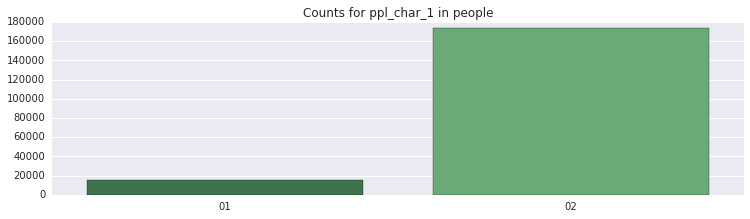
\includegraphics{BarPlots_files/BarPlots_4_0.png}
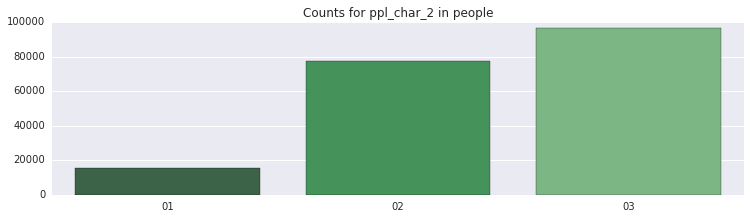
\includegraphics{BarPlots_files/BarPlots_5_0.png}
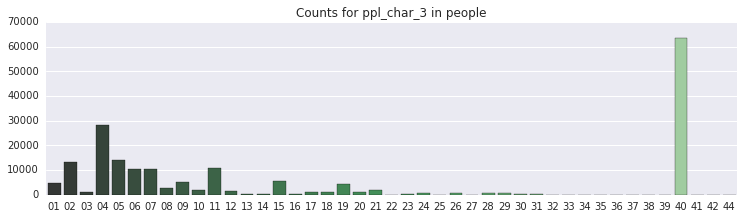
\includegraphics{BarPlots_files/BarPlots_5_1.png}
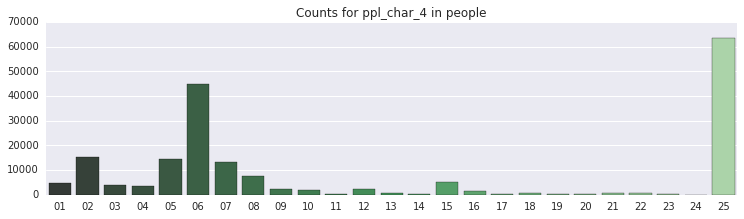
\includegraphics{BarPlots_files/BarPlots_5_2.png}
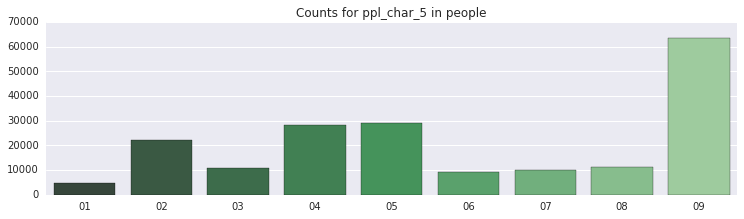
\includegraphics{BarPlots_files/BarPlots_5_3.png}
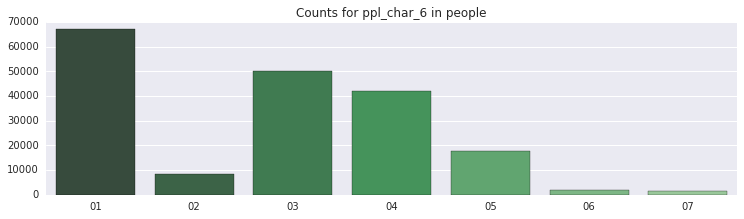
\includegraphics{BarPlots_files/BarPlots_5_4.png}
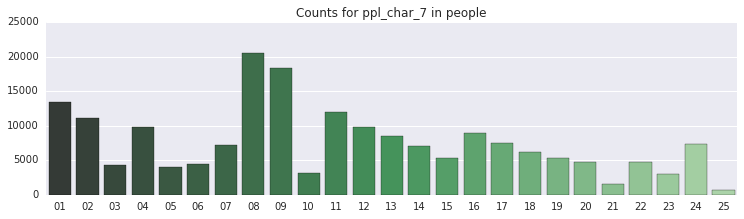
\includegraphics{BarPlots_files/BarPlots_5_5.png}
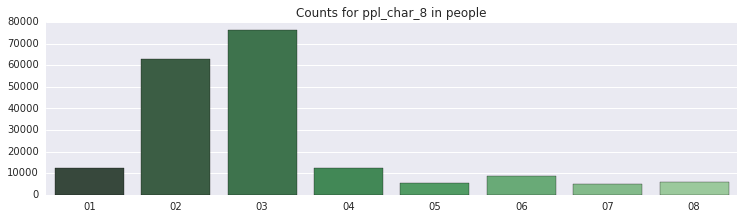
\includegraphics{BarPlots_files/BarPlots_5_6.png}
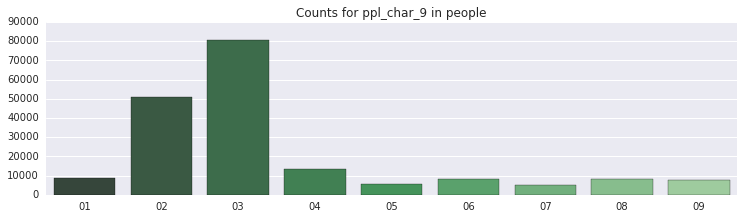
\includegraphics{BarPlots_files/BarPlots_5_7.png}
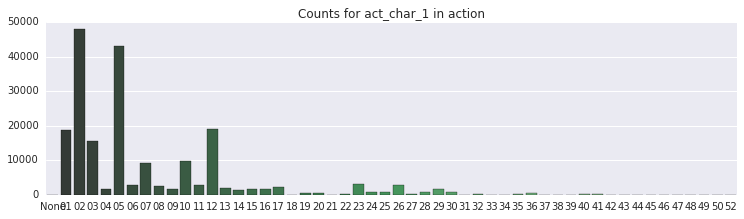
\includegraphics{BarPlots_files/BarPlots_6_0.png}
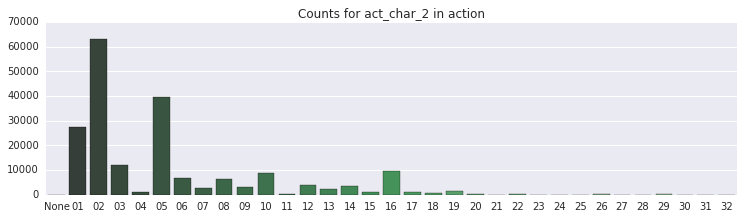
\includegraphics{BarPlots_files/BarPlots_6_1.png}
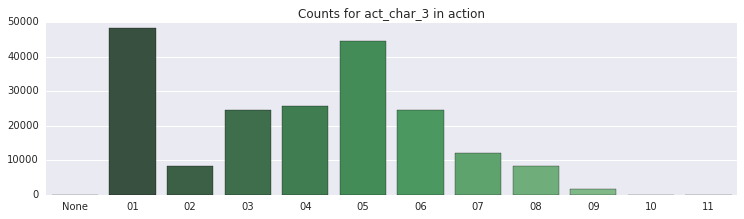
\includegraphics{BarPlots_files/BarPlots_6_2.png}
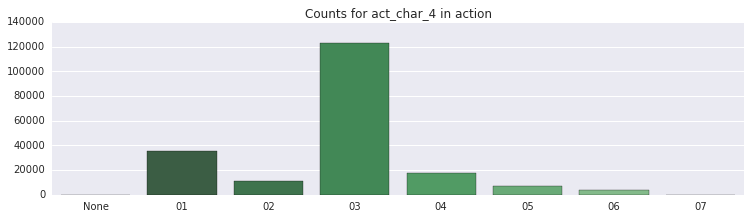
\includegraphics{BarPlots_files/BarPlots_6_3.png}
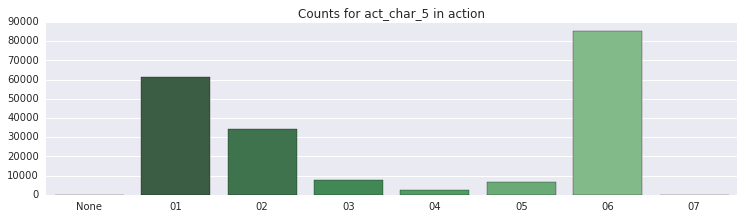
\includegraphics{BarPlots_files/BarPlots_6_4.png}
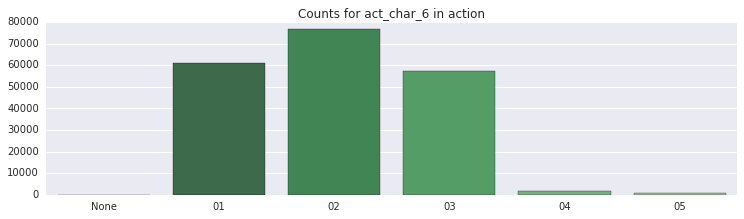
\includegraphics{BarPlots_files/BarPlots_6_5.png}
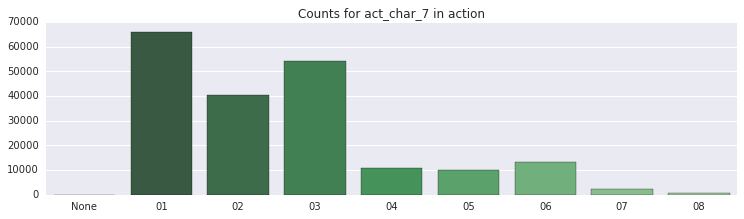
\includegraphics{BarPlots_files/BarPlots_6_6.png}
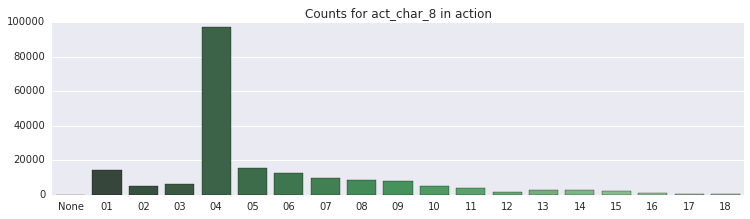
\includegraphics{BarPlots_files/BarPlots_6_7.png}
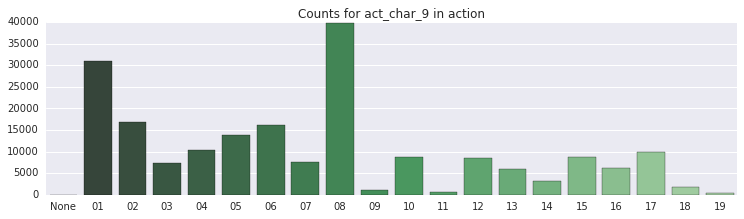
\includegraphics{BarPlots_files/BarPlots_6_8.png}

\pagebreak

\subsubsection{Exploratory
Visualization}\label{exploratory-visualization}

\textbf{TODO: we will need to one-hot encode to do this, i.e.~we are
going to do this visualization from data in the one-hot encoded table.}

\begin{Shaded}
\begin{Highlighting}[]
\CommentTok{# TODO: Apply PCA to the good data with the same number of dimensions as features}
\CharTok{from} \NormalTok{sklearn.decomposition }\CharTok{import} \NormalTok{PCA }
\NormalTok{pca = PCA(}\DecValTok{6}\NormalTok{)}
\NormalTok{pca.fit(good_data)}
\end{Highlighting}
\end{Shaded}

\begin{Shaded}
\begin{Highlighting}[]
\CommentTok{# create an x-axis variable for each pca component}
\NormalTok{x = np.arange(}\DecValTok{1}\NormalTok{,}\DecValTok{7}\NormalTok{)}

\CommentTok{# plot the cumulative variance}
\NormalTok{plt.plot(x, np.cumsum(pca.explained_variance_ratio_), }\StringTok{'-o'}\NormalTok{, color=}\StringTok{'black'}\NormalTok{)}

\CommentTok{# plot the components' variance}
\NormalTok{plt.bar(x, pca.explained_variance_ratio_, align=}\StringTok{'center'}\NormalTok{, alpha=}\FloatTok{0.5}\NormalTok{)}

\CommentTok{# plot styling}
\NormalTok{plt.ylim(}\DecValTok{0}\NormalTok{, }\FloatTok{1.05}\NormalTok{)}
\NormalTok{plt.annotate(}\StringTok{'Cumulative}\CharTok{\textbackslash{}n}\StringTok{explained}\CharTok{\textbackslash{}n}\StringTok{variance'}\NormalTok{,}
             \NormalTok{xy=(}\FloatTok{3.7}\NormalTok{, .}\DecValTok{88}\NormalTok{), arrowprops=}\DataTypeTok{dict}\NormalTok{(arrowstyle=}\StringTok{'->'}\NormalTok{), xytext=(}\FloatTok{4.5}\NormalTok{, .}\DecValTok{6}\NormalTok{))}
\KeywordTok{for} \NormalTok{i,j in }\DataTypeTok{zip}\NormalTok{(x, np.cumsum(pca.explained_variance_ratio_)):}
    \NormalTok{plt.annotate(}\DataTypeTok{str}\NormalTok{(j.}\DataTypeTok{round}\NormalTok{(}\DecValTok{4}\NormalTok{)),xy=(i}\FloatTok{+.2}\NormalTok{,j}\FloatTok{-.02}\NormalTok{))}
\NormalTok{plt.xticks(}\DataTypeTok{range}\NormalTok{(}\DecValTok{1}\NormalTok{,}\DecValTok{7}\NormalTok{))}
\NormalTok{plt.xlabel(}\StringTok{'PCA components'}\NormalTok{)}
\NormalTok{plt.ylabel(}\StringTok{'Explained Variance'}\NormalTok{)}
\NormalTok{plt.show()}
\end{Highlighting}
\end{Shaded}

\textbf{In this section, you will need to provide some form of
visualization that summarizes or extracts a relevant characteristic or
feature about the data. The visualization should adequately support the
data being used. Discuss why this visualization was chosen and how it is
relevant. Questions to ask yourself when writing this section:}

\begin{itemize}
\itemsep1pt\parskip0pt\parsep0pt
\item
  \emph{Have you visualized a relevant characteristic or feature about
  the dataset or input data?}
\item
  \emph{Is the visualization thoroughly analyzed and discussed?}
\item
  \emph{If a plot is provided, are the axes, title, and datum clearly
  defined?}
\end{itemize}

\pagebreak

\subsubsection{Algorithms and
Techniques}\label{algorithms-and-techniques}

\textbf{In this section, you will need to discuss the algorithms and
techniques you intend to use for solving the problem. You should justify
the use of each one based on the characteristics of the problem and the
problem domain. Questions to ask yourself when writing this section:}

\paragraph{One-Hot Encoding}\label{one-hot-encoding}

We will use the One-Hot Encoding algorithm to convert out our
categorical data to numerical data. We will use this algorithm in order
to convert our categorical data into numerical data. It may be tempting
to merely convert our categories to numbers i.e. \texttt{type 01} $\to$
1, \texttt{type 02} $\to$ 2, however, such an encoding of data implies a
linear relationship between our categories, where there may be none.

\begin{quote}
In one-hot encoding, a separate bit of state is used for each state. It
is called one-hot because only one bit is ``hot'' or TRUE at any time.
(Harris, David, and Sarah Harris. Digital design and computer
architecture. Elsevier, 2012.)
\end{quote}

This algorithm is also referred to as 1-of-K encoding. An example will
be helpful in illustrating the concept.

\begin{Shaded}
\begin{Highlighting}[]
\CharTok{import} \NormalTok{psycopg2}
\CharTok{import} \NormalTok{numpy }\CharTok{as} \NormalTok{np}
\CharTok{from} \NormalTok{os }\CharTok{import} \NormalTok{environ}
\NormalTok{conn = psycopg2.}\OtherTok{connect}\NormalTok{(dbname=}\StringTok{'postgres'}\NormalTok{, user=}\StringTok{'postgres'}\NormalTok{, host=environ[}\StringTok{'POSTGRES_1_PORT_5432_TCP_ADDR'}\NormalTok{])}
\NormalTok{cur = conn.cursor()}

 \NormalTok{cur.execute(}\StringTok{"SELECT ppl_char_1,ppl_char_2 FROM people LIMIT 10"}\NormalTok{)}
\NormalTok{this_row = cur.fetchone()}
\NormalTok{one_hot = []}
\KeywordTok{while} \NormalTok{this_row:}
    \NormalTok{one_hot.append([}
            \NormalTok{this_row[}\DecValTok{0}\NormalTok{] == }\StringTok{'type 1'}\NormalTok{,}
            \NormalTok{this_row[}\DecValTok{0}\NormalTok{] == }\StringTok{'type 2'}\NormalTok{,}
            \NormalTok{this_row[}\DecValTok{1}\NormalTok{] == }\StringTok{'type 1'}\NormalTok{,}
            \NormalTok{this_row[}\DecValTok{1}\NormalTok{] == }\StringTok{'type 2'}\NormalTok{,}
            \NormalTok{this_row[}\DecValTok{1}\NormalTok{] == }\StringTok{'type 3'}\NormalTok{,}
        \NormalTok{])}
    \NormalTok{this_row = cur.fetchone()}
\DataTypeTok{print}\NormalTok{(np.array(one_hot, dtype=}\DataTypeTok{int}\NormalTok{))}

\NormalTok{[[}\DecValTok{0} \DecValTok{1} \DecValTok{0} \DecValTok{1} \DecValTok{0}\NormalTok{]}
 \NormalTok{[}\DecValTok{0} \DecValTok{1} \DecValTok{0} \DecValTok{0} \DecValTok{1}\NormalTok{]}
 \NormalTok{[}\DecValTok{0} \DecValTok{1} \DecValTok{0} \DecValTok{0} \DecValTok{1}\NormalTok{]}
 \NormalTok{[}\DecValTok{0} \DecValTok{1} \DecValTok{0} \DecValTok{0} \DecValTok{1}\NormalTok{]}
 \NormalTok{[}\DecValTok{0} \DecValTok{1} \DecValTok{0} \DecValTok{0} \DecValTok{1}\NormalTok{]}
 \NormalTok{[}\DecValTok{0} \DecValTok{1} \DecValTok{0} \DecValTok{0} \DecValTok{1}\NormalTok{]}
 \NormalTok{[}\DecValTok{0} \DecValTok{1} \DecValTok{0} \DecValTok{1} \DecValTok{0}\NormalTok{]}
 \NormalTok{[}\DecValTok{0} \DecValTok{1} \DecValTok{0} \DecValTok{0} \DecValTok{1}\NormalTok{]}
 \NormalTok{[}\DecValTok{0} \DecValTok{1} \DecValTok{0} \DecValTok{0} \DecValTok{1}\NormalTok{]}
 \NormalTok{[}\DecValTok{0} \DecValTok{1} \DecValTok{0} \DecValTok{0} \DecValTok{1}\NormalTok{]]}
 
\end{Highlighting}
\end{Shaded}

Here, we select two columns from our database. For each available type
for each column, we do a Boolean check and then cast this check to an
integer. The result is that for a given group of columns corresponding
to a single column in our original database, there will be a single
\texttt{1} and the remainder will be \texttt{0}. We use one-hot coding
because the categorical and boolean nature of the vast majority of our
data lends itself to this technique.

\paragraph{Linear Classifier}\label{linear-classifier}

Linear classification will be the core algorithm upon which we will
build our neural network classifier. We borrow heavily for this approach
from Andrej Karpathy's
\href{http://cs231n.github.io/linear-classify/}{notes} for his
Convolutional Neural Networks course:

\begin{quote}
The approach will have two major components: a \textbf{score function}
that maps the raw data to class scores, and a \textbf{loss function}
that quantifies the agreement between the predicted scores and the
ground truth labels.
\end{quote}

\subparagraph{Score Function}\label{score-function}

We will develop a score function that maps input vectors to class scores

\[f: \mathbb{R^D} \mapsto \mathbb{R}^2\]

where $D$ is the dimension of our one-hot encoded vectors and 2
represents the 2 classes of our binary classifier. Then,

\[f(x_i, W, b)=Wx_i+b=y\]

where $x_i$ is a particular input vector, $W$ is a matrix of weights
(dimension $2 \times n$), $b$ is a bias vector, and $y$ is a score
vector with a score for each class.

\begin{figure}[htbp]
\centering
\includegraphics{http://cs231n.github.io/assets/imagemap.jpg}
\end{figure}

Loss Function

Note that of the inputs to our score function we do not have control
over the $x_i$s. Instead, we must change $W$ and $b$ to match a set of
given $y$s. To do this we will define a loss function that measures our
performance. We will use one of the most common loss functions the
multiclass support vector machine. Here the loss for a given vector is

\[L_i=\sum_{j\neq y_i}\max(0,s_j-s_{y_i}+\Delta)\]

Here, $s$ is the vector result of our score function and $y_i$ is the
correct class. Our loss function computes a scalar value by comparing
each incorrect class score to the correct class score. We expect the
score of the correct class to be at least $\Delta$ larger than the score
of each incorrect class.

Regularization Penalty

It is possible that more than one set of weights could provide an
optimal response to our loss function. In order to prioritize the
smallest possible weights we will add a regularization penalty to our
loss function. Again we will go with a common technique and use the L2
norm.

\[R(W)=\sum_k\sum_lW^2_{k,l}\]

Additionally, including a regularizatiom penalty has the added benefit
of helping to prevent overfitting.

\subparagraph{Final Loss Function}\label{final-loss-function}

\[L=\frac{1}{N}\sum_iL_i+\lambda R(W)\]

Here, $\lambda$ is a hyper parameter to be fit by cross-validation and
$N$ is a batch size.

\subsubsection{Benchmark}\label{benchmark}

The quality of a solution to this task will be measured using the
following test error metric

\[\text{Ave}(I(y_i\neq\hat{y}_i))\]

Here, $I$ is an indicator function which yields 0 if the predicted
outcome ($\hat{y}_i$) matches the actual outcome ($y_i$). While the size
of the dataset (over 2 million rows in the action set) makes this
problem atypical, it is at the end of the day, a binary classification
problem. As such this simple metric is sufficient to measure our
accuracy.

Of note is that, while the outcome is clearly defined by the contest,
for the purposes of this project, we will be using a portion of the
training set as our benchmark.

\subsection{Methodology}\label{methodology}

\subsubsection{Data Preprocessing}\label{data-preprocessing}

As previously discussed, we will primarily be preprocessing our data via
the one-hot encoding algorithm, transforming our categorical and boolean
data into integer values in the set $\{0,1\}$ that will ultimately be
encoded as integer values in a numpy array. Furthermore, we have
designed a system that uses a queueing mechanism for the running of
delayed job. In this way, we can execute a processing of each row in a
join table between our \texttt{people} and \texttt{action} tables as
background processes and take advantage of as many cores as possible on
a given architecture.

methods written in python

queuing mechanism and delayed job processing

\begin{verbatim}
from os import chdir
chdir('../')

from lib.app import Q

import psycopg2
import numpy as np
from os import environ
conn = psycopg2.connect(dbname='postgres', 
                        user='postgres', 
                    host=environ['POSTGRES_1_PORT_5432_TCP_ADDR'])
cur = conn.cursor()

cur = conn.cursor()
cur.execute("SELECT act_id FROM action WHERE act_outcome IS NOT NULL")

import lib.helpers.database_helper as dh

act_id = cur.fetchone()[0]
i = 0
while act_id and i < 1000 :
    Q.enqueue(dh.one_hot_encode_row, act_id)
    act_id = cur.fetchone()[0]
    i += 1
\end{verbatim}

\textbf{In this section, all of your preprocessing steps will need to be
clearly documented, if any were necessary. From the previous section,
any of the abnormalities or characteristics that you identified about
the dataset will be addressed and corrected here. Questions to ask
yourself when writing this section:}

\begin{itemize}
\itemsep1pt\parskip0pt\parsep0pt
\item
  \emph{If the algorithms chosen require preprocessing steps like
  feature selection or feature transformations, have they been properly
  documented?}
\item
  \emph{Based on the \textbf{Data Exploration} section, if there were
  abnormalities or characteristics that needed to be addressed, have
  they been properly corrected?}
\item
  \emph{If no preprocessing is needed, has it been made clear why?}
\end{itemize}

\subsubsection{Implementation}\label{implementation}

In this section, the process for which metrics, algorithms, and
techniques that you implemented for the given data will need to be
clearly documented. It should be abundantly clear how the implementation
was carried out, and discussion should be made regarding any
complications that occurred during this process. Questions to ask
yourself when writing this section: - \emph{Is it made clear how the
algorithms and techniques were implemented with the given datasets or
input data?} - \emph{Were there any complications with the original
metrics or techniques that required changing prior to acquiring a
solution?} - \emph{Was there any part of the coding process (e.g.,
writing complicated functions) that should be documented?}

\subsubsection{Refinement}\label{refinement}

In this section, you will need to discuss the process of improvement you
made upon the algorithms and techniques you used in your implementation.
For example, adjusting parameters for certain models to acquire improved
solutions would fall under the refinement category. Your initial and
final solutions should be reported, as well as any significant
intermediate results as necessary. Questions to ask yourself when
writing this section: - \emph{Has an initial solution been found and
clearly reported?} - \emph{Is the process of improvement clearly
documented, such as what techniques were used?} - \emph{Are intermediate
and final solutions clearly reported as the process is improved?}

\subsection{IV. Results}\label{iv.-results}

\emph{(approx. 2-3 pages)}

\subsubsection{Model Evaluation and
Validation}\label{model-evaluation-and-validation}

In this section, the final model and any supporting qualities should be
evaluated in detail. It should be clear how the final model was derived
and why this model was chosen. In addition, some type of analysis should
be used to validate the robustness of this model and its solution, such
as manipulating the input data or environment to see how the model's
solution is affected (this is called sensitivity analysis). Questions to
ask yourself when writing this section: - \emph{Is the final model
reasonable and aligning with solution expectations? Are the final
parameters of the model appropriate?} - \emph{Has the final model been
tested with various inputs to evaluate whether the model generalizes
well to unseen data?} - \emph{Is the model robust enough for the
problem? Do small perturbations (changes) in training data or the input
space greatly affect the results?} - \emph{Can results found from the
model be trusted?}

\subsubsection{Justification}\label{justification}

In this section, your model's final solution and its results should be
compared to the benchmark you established earlier in the project using
some type of statistical analysis. You should also justify whether these
results and the solution are significant enough to have solved the
problem posed in the project. Questions to ask yourself when writing
this section: - \emph{Are the final results found stronger than the
benchmark result reported earlier?} - \emph{Have you thoroughly analyzed
and discussed the final solution?} - \emph{Is the final solution
significant enough to have solved the problem?}

\subsection{V. Conclusion}\label{v.-conclusion}

\emph{(approx. 1-2 pages)}

\subsubsection{Free-Form Visualization}\label{free-form-visualization}

In this section, you will need to provide some form of visualization
that emphasizes an important quality about the project. It is much more
free-form, but should reasonably support a significant result or
characteristic about the problem that you want to discuss. Questions to
ask yourself when writing this section: - \emph{Have you visualized a
relevant or important quality about the problem, dataset, input data, or
results?} - \emph{Is the visualization thoroughly analyzed and
discussed?} - \emph{If a plot is provided, are the axes, title, and
datum clearly defined?}

\subsubsection{Reflection}\label{reflection}

In this section, you will summarize the entire end-to-end problem
solution and discuss one or two particular aspects of the project you
found interesting or difficult. You are expected to reflect on the
project as a whole to show that you have a firm understanding of the
entire process employed in your work. Questions to ask yourself when
writing this section: - \emph{Have you thoroughly summarized the entire
process you used for this project?} - \emph{Were there any interesting
aspects of the project?} - \emph{Were there any difficult aspects of the
project?} - \emph{Does the final model and solution fit your
expectations for the problem, and should it be used in a general setting
to solve these types of problems?}

\subsubsection{Improvement}\label{improvement}

In this section, you will need to provide discussion as to how one
aspect of the implementation you designed could be improved. As an
example, consider ways your implementation can be made more general, and
what would need to be modified. You do not need to make this
improvement, but the potential solutions resulting from these changes
are considered and compared/contrasted to your current solution.
Questions to ask yourself when writing this section: - \emph{Are there
further improvements that could be made on the algorithms or techniques
you used in this project?} - \emph{Were there algorithms or techniques
you researched that you did not know how to implement, but would
consider using if you knew how?} - \emph{If you used your final solution
as the new benchmark, do you think an even better solution exists?}

\begin{center}\rule{3in}{0.4pt}\end{center}

\textbf{Before submitting, ask yourself. . .}

\begin{itemize}
\itemsep1pt\parskip0pt\parsep0pt
\item
  Does the project report you've written follow a well-organized
  structure similar to that of the project template?
\item
  Is each section (particularly \textbf{Analysis} and
  \textbf{Methodology}) written in a clear, concise and specific
  fashion? Are there any ambiguous terms or phrases that need
  clarification?
\item
  Would the intended audience of your project be able to understand your
  analysis, methods, and results?
\item
  Have you properly proof-read your project report to assure there are
  minimal grammatical and spelling mistakes?
\item
  Are all the resources used for this project correctly cited and
  referenced?
\item
  Is the code that implements your solution easily readable and properly
  commented?
\item
  Does the code execute without error and produce results similar to
  those reported?
\end{itemize}

\subsection{Appendix}\label{appendix}

\textless{}a \#\#\# \texttt{Dockerfile}

\begin{verbatim}
# docker/postgres/Dockerfile
FROM postgres
COPY tables.sql /docker-entrypoint-initdb.d/tables.sql
COPY act_test.csv /docker-entrypoint-init.d/act_test.csv
COPY act_train.csv /docker-entrypoint-init.d/act_train.csv
COPY people.csv /docker-entrypoint-init.d/people.csv
\end{verbatim}

\subsubsection{}\label{section}

\end{document}
